\section{Matched Objective and Feedback-History Comparison}
\label{sec:native-longitudinal-comparison}

\paragraph{Question, authority and finite design.}
The next study compares scalar feedback with access to the parent's native
trajectory under throughput loss $L_T$ and common-content utility loss $L_U$.
The searched object remains the organizing institution: both information arms
can edit executable rules, mechanisms, wiring and schedules. They retain the
original four-year persistent researcher world, corpus, fixed Qwen3-8B
researchers and approved local 35B designer. Each of four own histories receives
three proposal slots, for twelve total. Seed 61001 is reused across this
development comparison; neither candidates nor feedback steps are independent
optimizer replications. The original reference is optimizer-visible; the
developer-authored post-funding-cost comparison is withheld from the designer.
Here R7 is the developer-authored seed institution, not the published
simulator's unmodified default institutional configuration; the original native
researcher engine is retained while the organizing institution is editable.
Losses, technical validity and held-out evaluation remain separate concepts.

\begin{table}[t]
\centering
\small
\begin{tabular}{llrrr}
\toprule
Feedback & Assigned loss & G0 & G1 & G2 \\
\midrule
Scalar & $L_T$ & $-18$ & $-18$ & null \\
Parent trajectory & $L_T$ & $-18$ & $-18$ & $-18$ \\
Scalar & $L_U$ & $-13.33$ & $-13.33$ & $-13.33$ \\
Parent trajectory & $L_U$ & $-13.33$ & null & $-13.33$ \\
\bottomrule
\end{tabular}
\caption{All twelve scheduled own slots; smaller loss is better. Utility is
rounded here from $-13.333333333333332$. Ten measured assigned losses tie the
original reference. The hand comparison achieves $L_T=-20$, $L_U=-15.33$.
Nulls are unknown losses after native runtime failures, not assigned penalties
or silently replaced samples. One reused development condition supplies no
independent error bars or isolated information-condition effect.}
\label{tab:longitudinal-all-slots}
\end{table}

\paragraph{Closed paths, without improvement.}
All twelve proposals are submitted; ten complete native measurements and two
fail at the publication consumer. There is no generation error, host source
repair, failed-slot refill, novelty requirement, fairness veto or loss change.
Every measured assigned loss ties the original reference and is worse than the
hand comparison by 2. Nine own candidates share the original cross-score vector,
$L_T=-18$, $L_U=-13.333333333333332$. Final parent-trajectory T2 instead has
$L_T=-18$, $L_U=-12.333333333333332$: matching its assigned throughput target
does not mean unchanged cross-objective behavior or improved utility.

\begin{figure}[t]
\centering
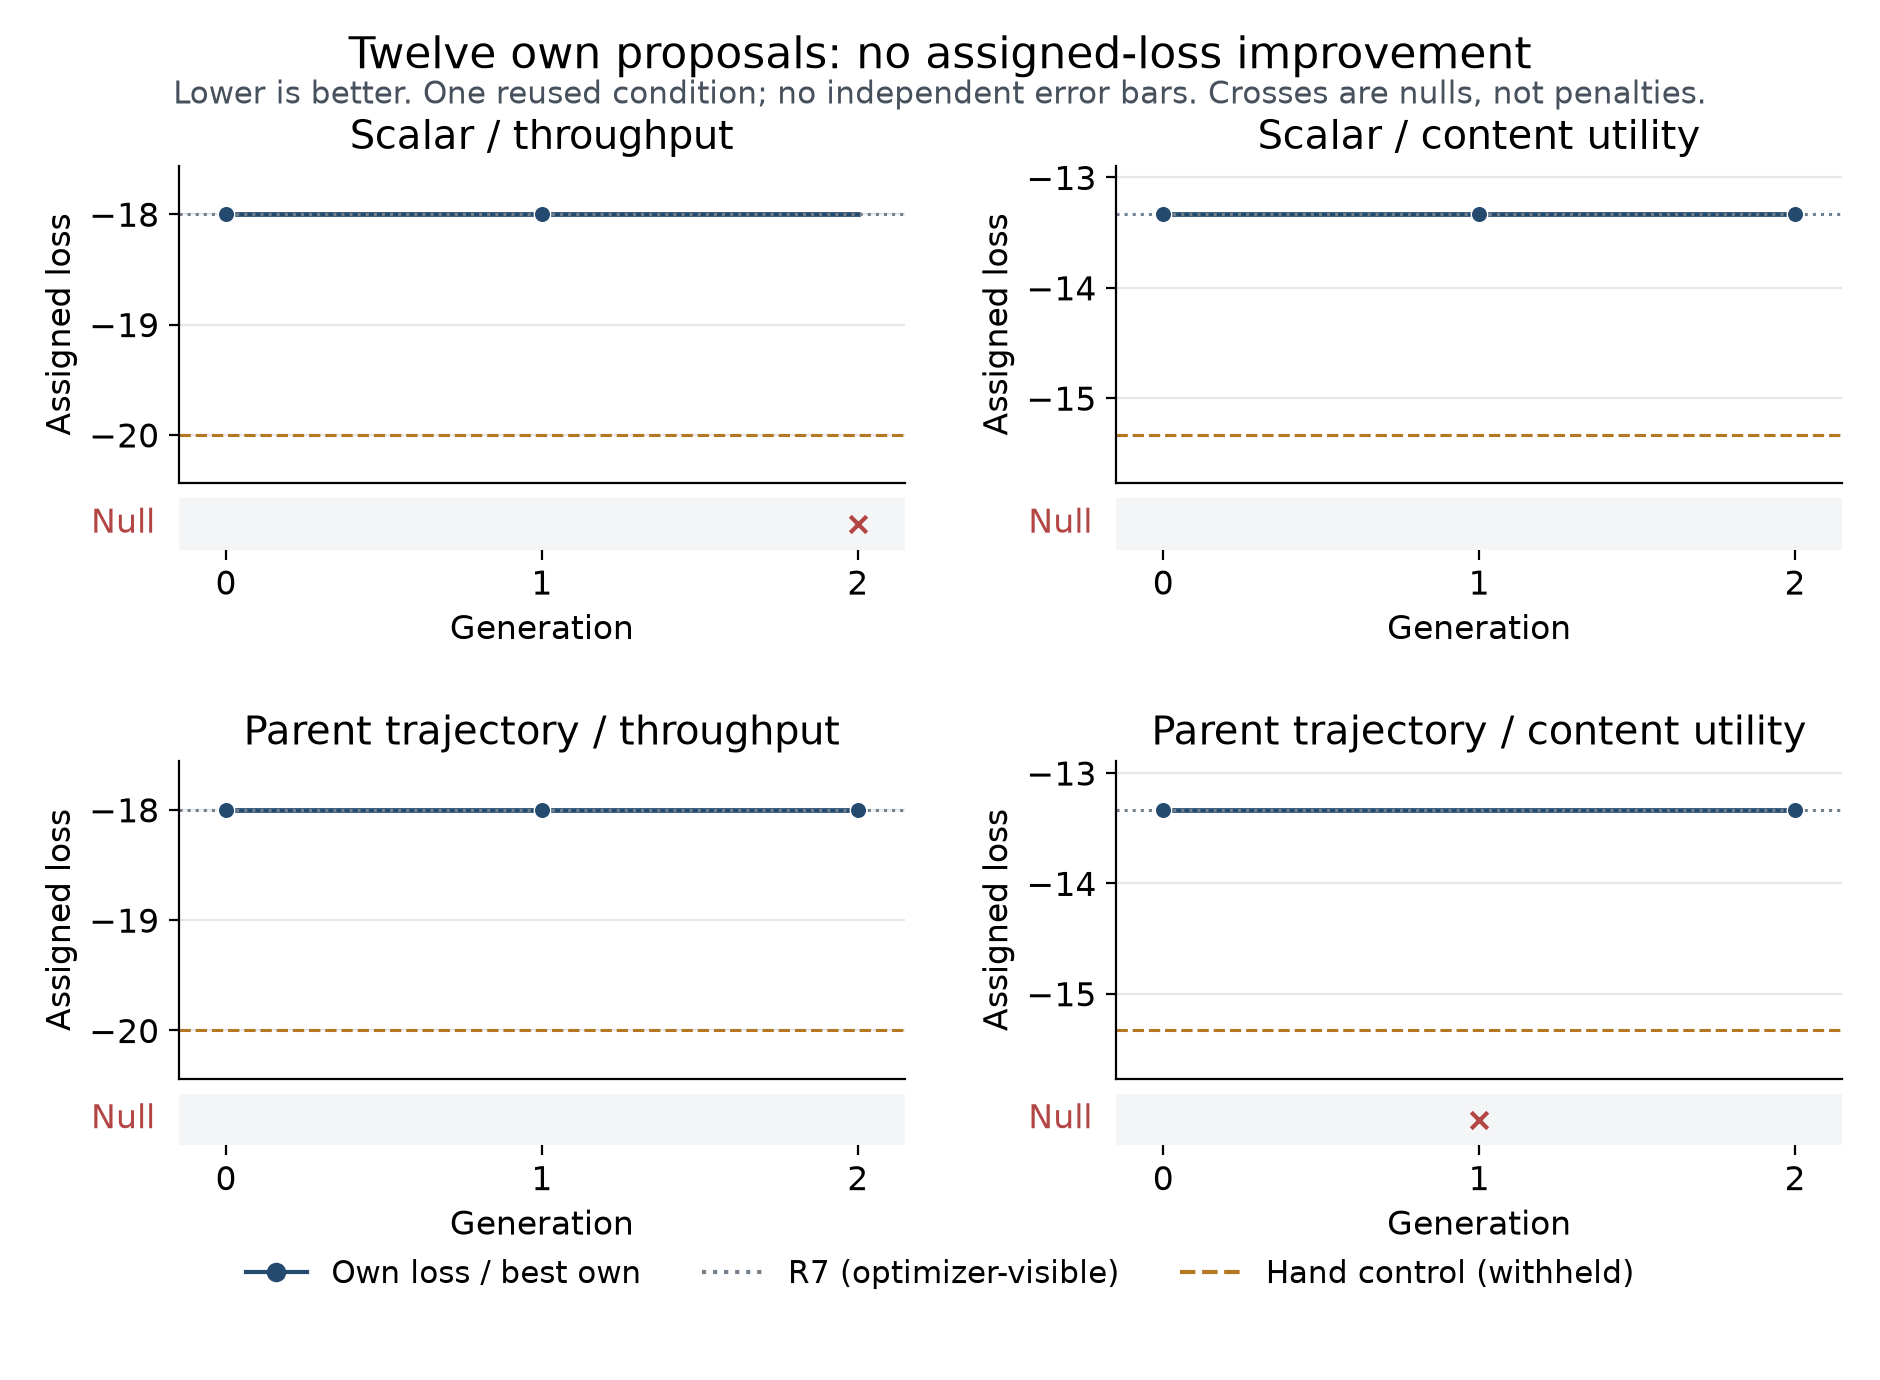
\includegraphics[width=\linewidth]{figures/native-longitudinal-development-print-v2/assigned-loss-paths-print.png}
\caption{Complete assigned-loss paths in the matched comparison. Dots are
completed proposals; lines carry forward the best own measured loss. Crosses
occupy a separate nonnumeric null strip, not the loss axis. The original R7
reference is optimizer-visible; the hand comparison is withheld. Cross-objective
worsening of final parent-trajectory T2 is reported in the text, not plotted
as its assigned throughput loss. One reused condition gives no independent
optimizer-replication error bars.}
\label{fig:longitudinal-assigned-paths}
\end{figure}

The finite measured matrix contains only three distinct T/U vectors: the
reference plus nine own worlds, the hand, and final parent-trajectory T2.
The hand strictly dominates every other measured row in both recorded losses.
Any nonzero nonnegative linear weighting of these two losses therefore keeps
it best within this measured set. This does not identify a global or expected
Pareto frontier. Nor does the absence of a preference reversal establish that
objectives do not matter: the search has not generated a measured tradeoff
on which to test objective-conditioned institutional choice.

\paragraph{Source diversity is not behavioral diversity.}
The complete journals contain 168 charged author steps and 108 component probes;
every probe returns, but those producer probes do not execute the complete
downstream publication contract. All 27 document-changing operations address
\code{world.selection}. Ten submitted systems change selection source relative
to the reference, while two retain it literally. None adds or removes a node,
connection or schedule or changes another system field. The existing file API
supports complete authored nodes and root-level composition edits, so these
results do not establish that structural invention is unavailable in the
representation. They show that this finite local search did not produce it.

Final-checkpoint inspection finds zero rejected records in every completed
world: 18 accepted in the reference and each valid own world, 20 in the hand
comparison. Accepting every paper already saturates immediate throughput on
each actually recorded decision batch. Concentration in selection edits thus
targets a stage with no immediate fixed-batch acceptance headroom. In contrast,
the hand changes timing/routing and the eventual submission volume. This is
not a global throughput bound or proof of the author's search bias: another
decision could alter later information, resources or submission batches.

Cold comparison of full scientist request payloads, rather than source hashes
or scalar losses alone, places the reference and nine valid own worlds in one
exact observed-input class. Their literal response choices also agree; full
provider envelopes do not all agree. The last valid proposal and hand comparison
each have a different full input sequence. Failed worlds do not become complete
path-equivalence classes. This is observed-path equivalence under a shared
condition, not global policy equivalence, independent replication or permission
to deduplicate nonidentical systems in subsequent evaluation.

\paragraph{An operative score route without an assigned-loss gain.}
The final valid proposal accepts real submitted papers with constant
\code{final\_score}=1. Its first 70 scientist request payloads match the reference.
Request 71 (index 70), a year 4 round-intention prompt, first differs in delivered
own-history dossier review scores and native past-paper scores, 0.0 versus 1.0.
The complete text difference consists of six changed digits: four dossier
fields and two \emph{Your Past Papers} scores. The actual consumer copies the
authored final score into the paper; publication archives it in review history,
and both the information office and native past-paper prompt renderer read
that archive into researcher context.
Thus a score absent from the direct critic-loss formula can still be operative
through future information. Declaring it inert from the loss formula alone
would miss this path.

Both worlds accept 18 content occurrences. Fourteen common year/content pairs
have identical retained content and critic values. Four reference-only pairs
contribute 4 centered utility units, whereas four last-proposal-only pairs
contribute 3, accounting exactly for the utility worsening by 1. Annual author
accounting, final-active count 2 and final resources 40 match. This is a decomposition
of one coupled trajectory, not a score-only average causal effect, scientific
truth measurement or policy-general welfare conclusion.

\paragraph{The two nulls expose a producer/consumer boundary.}
Parent-trajectory U1 returns a scored empty-cycle marker instead of the exact
explicit empty decision batch. Scalar T2 double-wraps already wrapped decisions.
Both reach and fail the unchanged native empty-cycle consumer contract. Their
losses remain unknown. Returning successfully from a component probe is not
whole-world validity. Regression cases cover the observed shapes without
repairing these historical candidates or unwrapping their decisions on the host.

\paragraph{Costs and frozen evaluation.}
The original runner closes normally after 5h56m39.98s on the shared host.
This is not a dedicated inference benchmark or the project's total cost.
The cost reader records 1,391 completed scientist responses and 84 separate
physical common-content observer requests, all 84 with known terminal attempts.
Auxiliary groups retain 372 editor-readiness attempts, 168 staged proposal
attempts, 25 designer-load attempts and 14 scientist-load attempts. Readiness
and proposal transport intervals total 6,401.32s and 5,708.03s respectively;
they are operations inside, not additions to, overall elapsed time. One of 168
proposal records lacks the final-response flag despite a retained HTTP record;
HTTP completion is not conflated with explicit finished designs or native worlds.
Missing usage is not imputed, overlapping durations are not added and response
records are not treated as additional independent scientific observations.

Two original-source cold audits and cost reports match byte for byte. Each of
five paired readout file sets and the paired allocation reports also matches.
These are reconstructions of one experiment, not repeated inference. The
original own-only minimum and earliest-tie rule selects generation 0 in every
history, with no hand-policy fallback. Reserved seed 676047151 supplies the
predeclared unused condition after broad source-bound usage inventories.
Four frozen own selections and two references share five physical jobs solely
through literal system identity, with zero new designer-generation POSTs.
\paragraph{Closed unused-condition outcomes.}
All five physical jobs complete normally on reserved seed 676047151
(Table~\ref{tab:longitudinal-fixed}; Figure~\ref{fig:longitudinal-fixed}).
The original reference and every frozen own selection yield 34 accepted records
and centered content-opinion utility 25.666666666666668; the hand yields 36 and 30.
Thus each selected institution ties R7 but has loss differences of $+2$ on T
and $+13/3$ on U against the hand. No candidate is selected again, repaired or
substituted using these results. All five cold initial physical-society
identities agree. The four distinct own/R7 physical worlds also share an exact
full scientist request sequence and literal response choices; complete provider
envelopes are not all equal. Sharing the one literal-identical R7/scalar-U
job is a separate fact from this observed-path equality.

\begin{table}[t]
\centering
\small
\begin{tabular}{lrrc}
\toprule
Frozen label & $L_T$ & $L_U$ & Physical job \\
\midrule
R7 reference & $-34$ & $-25.67$ & 000 \\
Hand reference & $-36$ & $-30$ & 001 \\
Scalar / T selection & $-34$ & $-25.67$ & 002 \\
Scalar / U selection & $-34$ & $-25.67$ & 000 \\
Parent trajectory / T selection & $-34$ & $-25.67$ & 003 \\
Parent trajectory / U selection & $-34$ & $-25.67$ & 004 \\
\bottomrule
\end{tabular}
\caption{All six frozen logical labels on the single reserved unused condition.
Job 000 is shared only because the complete policies are literally identical.
The other jobs execute separately despite their observed input equality.
Utility is rounded from 25.666666666666668. These are not six independent
replications, and the condition never enters the historical optimizer bank.}
\label{tab:longitudinal-fixed}
\end{table}

\begin{figure}[t]
\centering
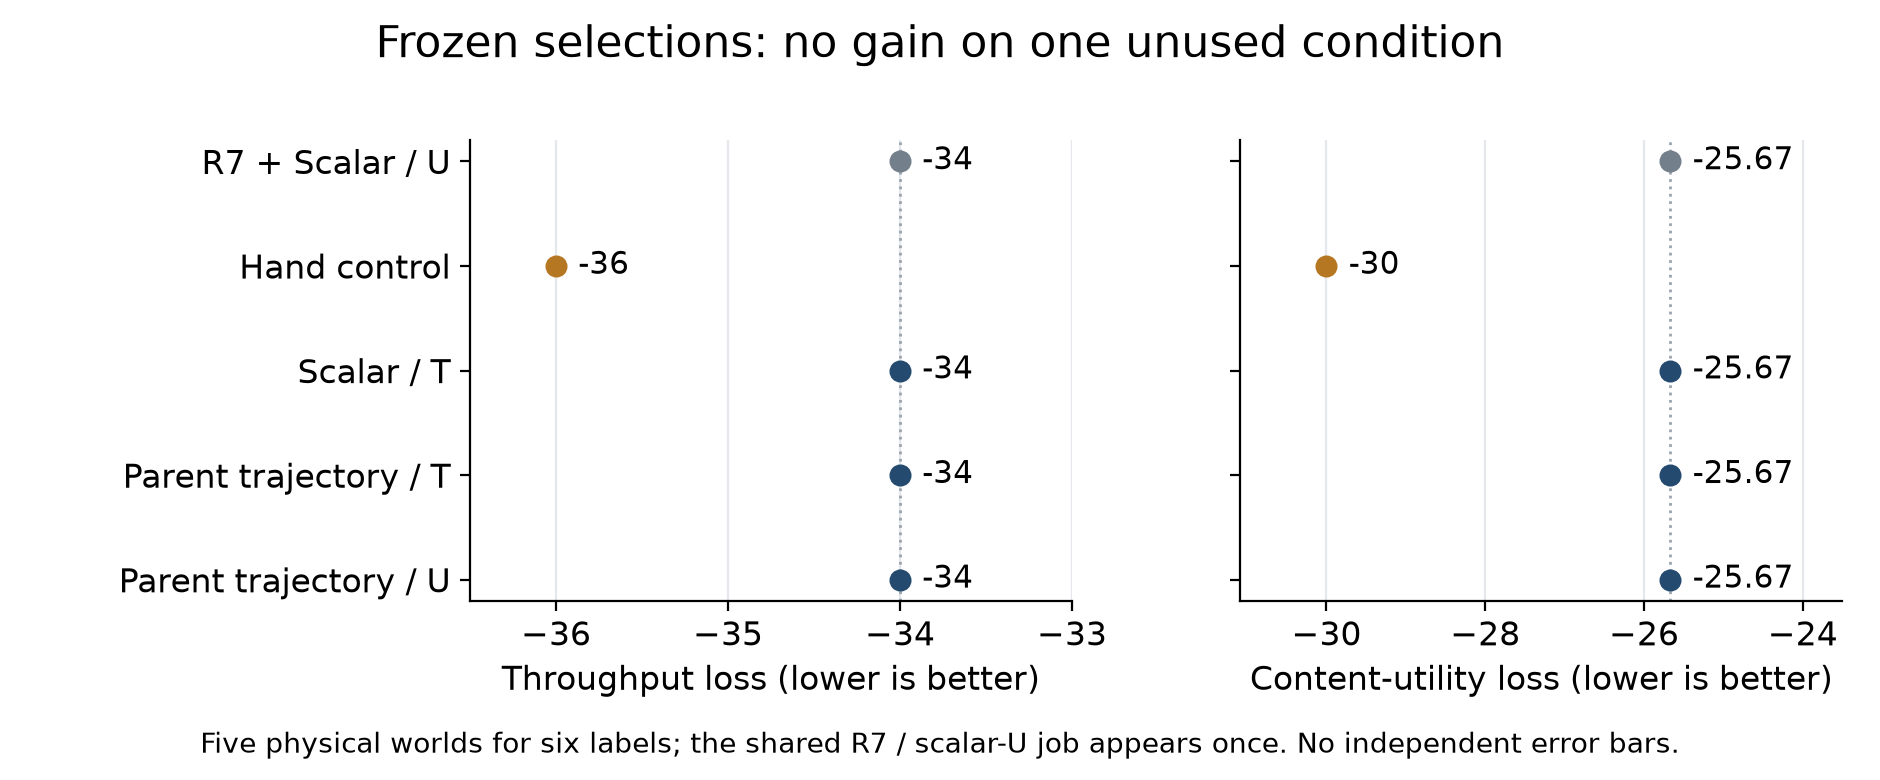
\includegraphics[width=\linewidth]{figures/native-longitudinal-fixed-print-v1/fixed-policy-scores-print.png}
\caption{Frozen evaluation shown once per physical job. R7 and the scalar-U
selection share the top row; the remaining selected programs execute separately.
Lower loss is better. The additional trajectory-access condition does not yield
an observed gain here. This single unused condition is neither an independent
optimizer replication nor a statement of expected superiority or equivalence.}
\label{fig:longitudinal-fixed}
\end{figure}

The hand/reference content difference is not merely two additional records.
Their 28 common year/paper occurrences have identical frozen critic values and
contribute $68/3$ utility units. Six R7-only occurrences contribute 3; eight
hand-only occurrences contribute $22/3$. The net utility difference is therefore
$22/3-3=13/3$. This exact fixed-record decomposition uses shared content ratings,
not new critiques or scientific truth. The hand changes timing and information
routing jointly, so this is not an isolated timing-effect estimate.

The fixed runner takes 1h09m35.57s on the shared host, separately from development.
It records 825 completed scientist responses, 126 physical common-observer POSTs
and five empty scientist-load attempts; there are zero designer-generation POSTs.
Scientist provider usage reports 1,305,668 prompt and 78,658 completion tokens
(1,384,326 total); 191,272 cached-prompt tokens are a reported subset, not extra
tokens added to that total. Two original-source audits and cost reports match,
as do paired score, full-input, project-choice and mechanism-effect readouts.
No successful reconstruction creates another independent scientific sample.

Unused evaluation does not revise the earlier selections or establish a causal
benefit of trajectory access. These tied and adverse outcomes locate the limits
of this finite search without showing that
objectives never matter, that broader institution search is impossible, or
that the project is main-track publication-ready.
